\begin{Methode}[Étude de signe d'un trinôme donné sous forme factorisée]
    Pour étudier le signe d'un polynôme de degré 2 donné sous forme factorisée, il faut dresser un tableau de signes dans lequel :
    \vspace{-0.3cm}\begin{tcbenumerate}[2]
        \tcbitem Chaque ligne est liée à un facteur. 
        \tcbitem Les signes de la ligne $f(x)$ sont déterminés par la \acc{règle des signes}. 
    \end{tcbenumerate}
    \vspace{-0.3cm}Soit $f$ la fonction définie sur $\R$ par $f\colon x \longmapsto -5(x-5)(x+3)$. Le tableau de signe de $f$ est :
    \begin{center}
    \begin{tikzpicture}
    \tkzTabInit[espcl=2.5,lgt=2]{$x$/0.8,$-5$/0.8,$x-5$/0.8,$x+3$/0.8,$f(x)$/0.8}
    {$-\infty$,$-3$,$5$,$+\infty$}
    \tkzTabLine{,-,t,-,t,-,}
    \tkzTabLine{,-,t,-,z,+,}
    \tkzTabLine{,-,z,+,t,+,}
    \tkzTabLine{,-,z,+,z,-,}
    \end{tikzpicture}
    \end{center}
\end{Methode}